\\ \textbf{Question 3.} \\
\hrule 
Three components are connected to form a system as shown in the accompanying diagram. Because the components in the 2-3 subsystem are connected in parallel, that subsystem will function if at least one of the two individual components function. For the entire system to function, component 1 must function and so must the 2-3 subsystem. \smallskip

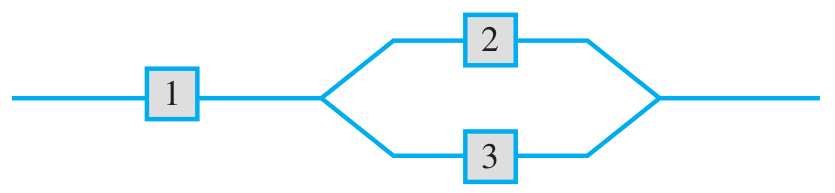
\includegraphics[scale=0.25]{images/whw3/2.1.3_diagram.png} \smallskip

The experiment consists of determining the condition of each component [$S$ (success) for functioning component and $F$ (failure) for a non-functioning component.] \smallskip

\textbf{a. Which outcomes are contained in the event $A$ that exactly two of the three components function?} \newline 
The following outcomes have exactly two functioning components.
\[ A = \{SSF, FSS, SFS\} \] \medskip

\textbf{b. Which outcomes are contained in the event $B$ that at least two of the components function?} \newline
The following outcomes have at least two functioning components.
\[B = \{ SSF, FSS, SSS, SFS\} \] \medskip 

\textbf{c. Which outcomes are contained in the event $C$ that the system functions?} \newline
The following outcomes allow the system to function.
\[ C = \{ SFS, SSF, SFS \} \] \medskip

\textbf{d. List outcomes in $C', A \cup C, A \cap C, B \cup C, \text{and} \; B \cap C$.}
\begin{align*}
C' &= \{ SFF, FFF, FFS, FSF \} \\
A \cup C &= \{ SSF, FSS, SFS, SSS \} \\
A \cap C &= \{ SSF, SFS \} \\
B \cup C &= \{ SSF, FSS, SSS, SFS\} \\
A \cap C &= \{ SSS, SSF, SFS \}
\end{align*}